\documentclass[11pt]{article}
\usepackage[utf8]{inputenc}
\usepackage[T1]{fontenc}
\usepackage[margin=0.82in,headheight=15pt]{geometry}
\usepackage{lmodern}
\usepackage{amsmath,amssymb}
\usepackage{array}
\usepackage{booktabs}
\usepackage{graphicx}
\usepackage{enumitem}
\usepackage{xcolor}
\usepackage[hidelinks]{hyperref}
\usepackage{titlesec}
\usepackage{fancyhdr}

\setlength{\parindent}{0pt}
\setlength{\parskip}{0.44em}
\setlist[itemize]{nosep,leftmargin=1.35em}
\definecolor{Accent}{HTML}{0B4F6C}
\definecolor{Soft}{HTML}{F2F6FA}
\titleformat{\section}{\large\bfseries\color{Accent}}{}{0pt}{}
\titleformat{\subsection}{\normalsize\bfseries\color{Accent}}{}{0pt}{}
\pagestyle{fancy}
\fancyhf{}
\fancyhead[L]{Chaos Toolbox}
\fancyhead[R]{Explorador Sprott}
\fancyfoot[C]{\thepage}
\renewcommand{\arraystretch}{1.18}

\newcommand{\code}[1]{\texttt{#1}}

\begin{document}

{\LARGE\bfseries Teoria del Explorador Sprott}\par
{\small Documento compilado para la pestana \emph{Explorador Sprott > Teoria}.}\par
\vspace{0.8em}

\tableofcontents
\newpage

\section{Fuente y alcance}

La referencia principal es el libro de Julien C. Sprott,
\emph{Strange Attractors: Creating Patterns in Chaos} \cite{sprott1993book},
junto con el manuscrito oficial que Sprott mantiene en su sitio de la University
of Wisconsin \cite{sprott1993online}. Tambien se cita la galeria oficial de
Sprott \cite{sprottgallery} y su articulo sobre flujos caoticos simples
\cite{sprott1994flows}.

Chaos Toolbox no redistribuye figuras, ejecutables, diccionarios ni codigo
historico de Sprott. Las graficas de este documento son generadas localmente por
la toolbox con ecuaciones y parametros indicados.

\section{Idea central}

Sprott presenta el caos como una combinacion de determinismo, sensibilidad a
condiciones iniciales y acotamiento no trivial. Dos estados iniciales cercanos
pueden separarse de forma aproximadamente exponencial:
\[
\lVert x_n-y_n\rVert \approx \lVert x_0-y_0\rVert e^{\lambda n}.
\]

Para la exploracion computacional esto implica una regla de lectura:
\begin{itemize}
  \item una figura visualmente atractiva no prueba caos;
  \item una trayectoria irregular corta tampoco basta;
  \item un candidato util debe conservar codigo, ecuaciones, parametros,
        transitorio, grafica y diagnosticos.
\end{itemize}

\section{De reglas simples a formas complejas}

El ejemplo didactico basico es la ecuacion logistica:
\[
x_{n+1}=R x_n(1-x_n).
\]
Al variar \(R\), la orbita pasa de punto fijo a ciclos periodicos,
duplicaciones de periodo y regiones caoticas con ventanas periodicas.

\begin{figure}[htbp]
\centering
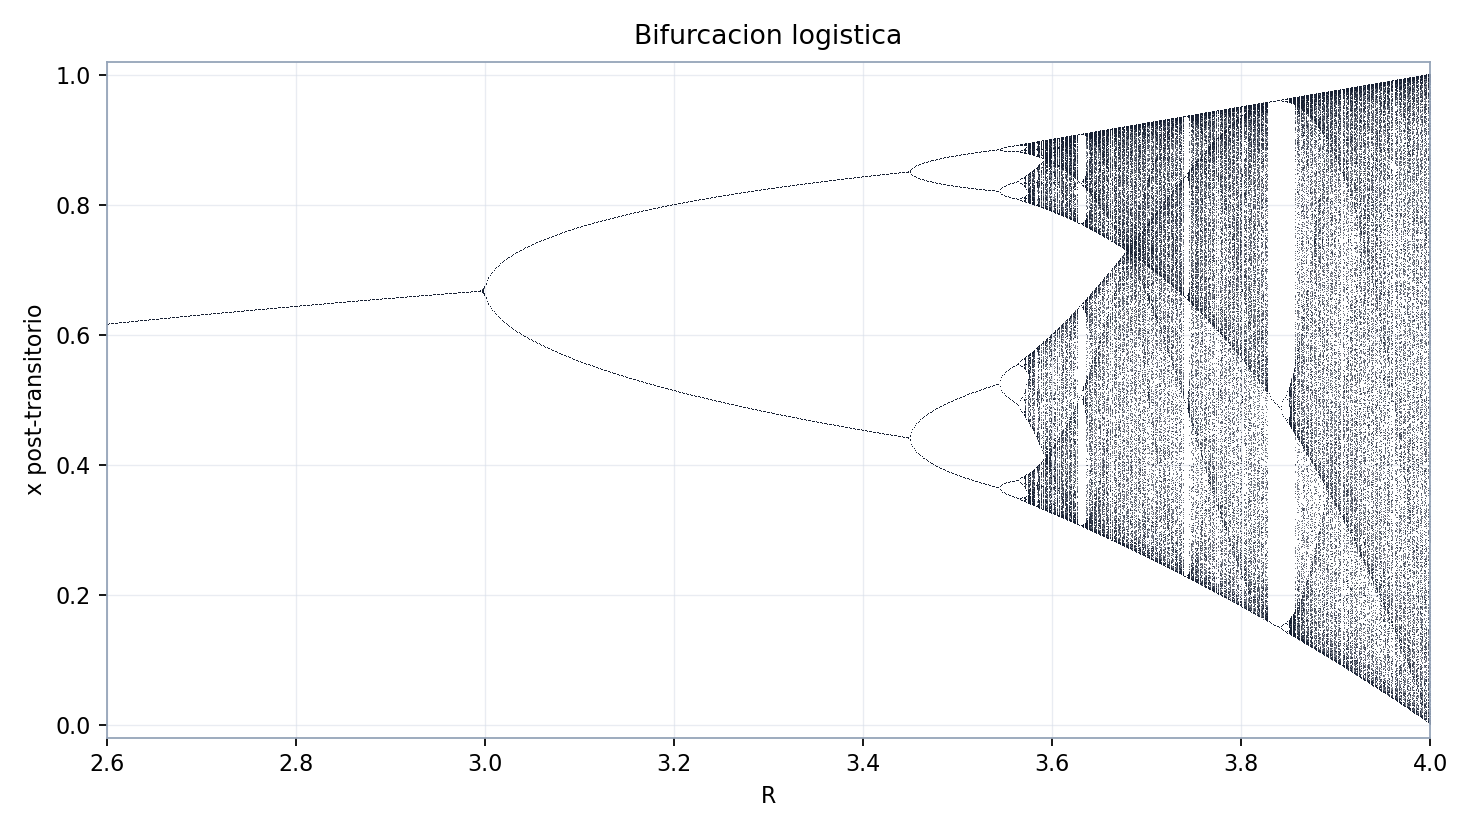
\includegraphics[width=0.92\linewidth]{images/logistic_bifurcation_sprott_theory.png}
\caption{Bifurcacion logistica generada por Chaos Toolbox con 1000 valores de
\(R\), 1200 iteraciones por valor y descarte de 700 iteraciones transitorias.}
\end{figure}

\section{Mapas polinomiales}

Un mapa discreto calcula directamente el siguiente estado:
\[
x_{n+1}=F(x_n), \qquad F_i(x)=\sum_j c_{ij}m_j(x).
\]
En dos dimensiones, cada iteracion produce un punto del plano. La no linealidad
puede contraer areas en unas direcciones y estirar en otras, generando objetos
que tienen mas detalle que una curva simple pero no llenan todo el plano.

\begin{figure}[htbp]
\centering
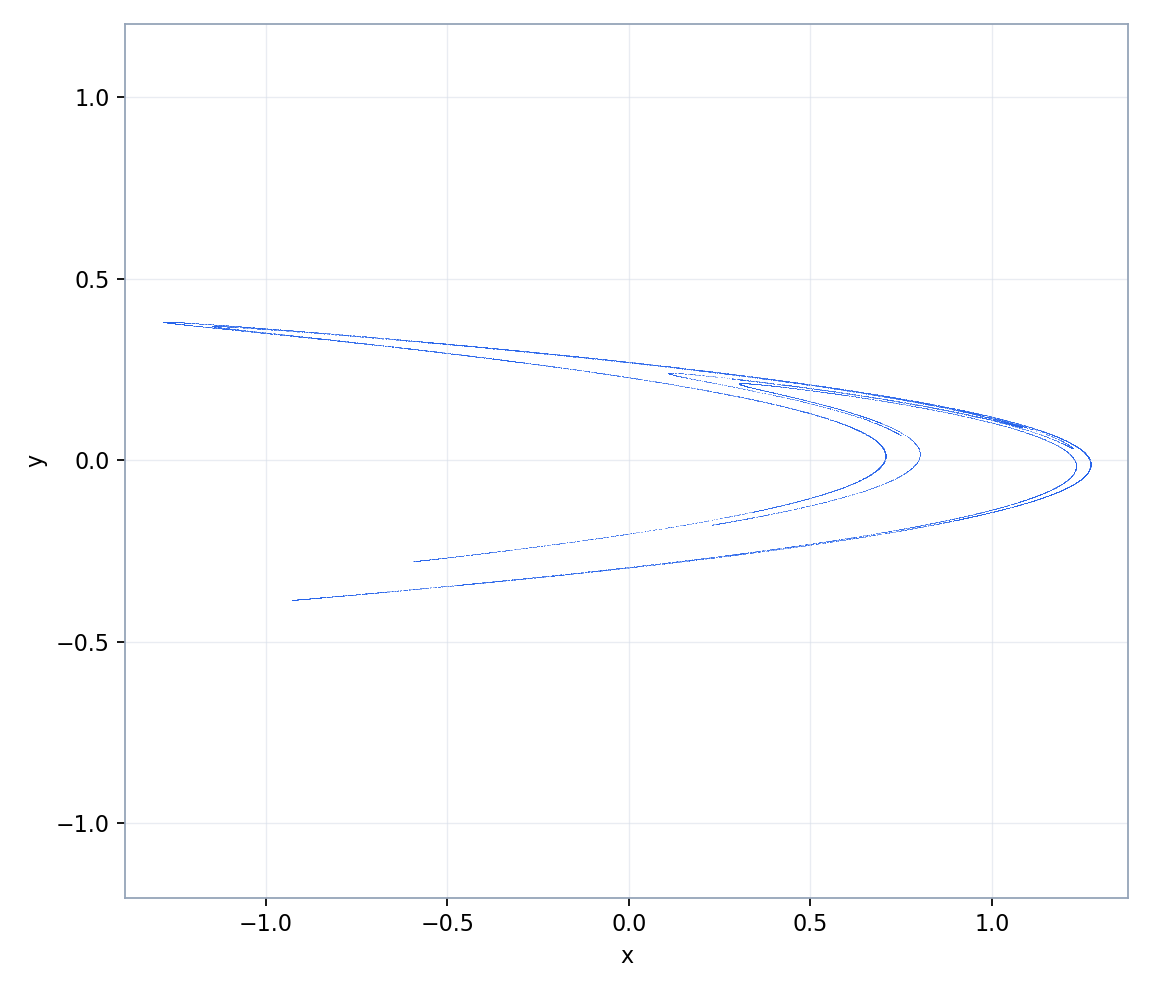
\includegraphics[width=0.72\linewidth]{images/henon_like_synthetic_sprott_theory.png}
\caption{Mapa de Henon generado con \(x'=1-1.4x^2+y\), \(y'=0.3x\), 26000
iteraciones y descarte de 1000.}
\end{figure}

\section{Flujos polinomiales}

Un flujo continuo define derivadas:
\[
\dot{x}=F(x), \qquad x(t+h)\approx x(t)+hF(x(t)).
\]
El capitulo de campos y flujos del libro conecta esta idea con Lorenz y Rossler.
Como ejemplo teorico, Sprott da un sistema tridimensional de cinco terminos:
\[
x'=yz,\qquad y'=x-y,\qquad z'=1-xy.
\]

\begin{figure}[htbp]
\centering
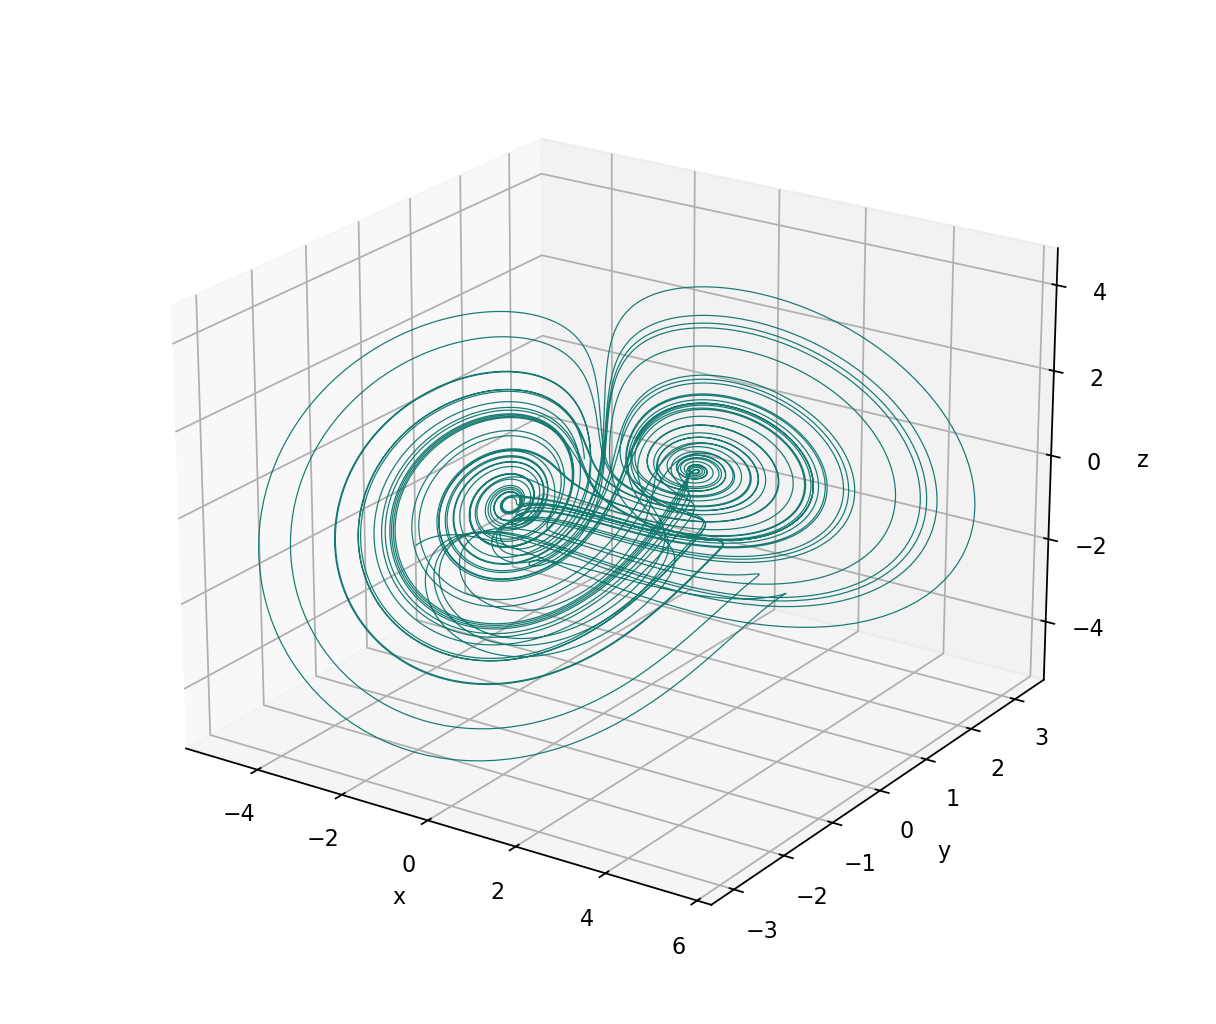
\includegraphics[width=0.74\linewidth]{images/sprott_five_term_flow_theory.png}
\caption{Flujo 3D de cinco terminos citado por Sprott, integrado con RK4,
\(h=0.01\), 60000 pasos y descarte de 10000.}
\end{figure}

\section{Lenguaje visual}

Las imagenes tipo Sprott no dependen solo de la ecuacion. La proyeccion, el
color por una coordenada oculta, el fondo, la opacidad y el numero de puntos
pueden revelar o esconder estructura.

\begin{figure}[htbp]
\centering

\includegraphics[width=0.48\linewidth]{images/generated/comparison_color_z_black.png}
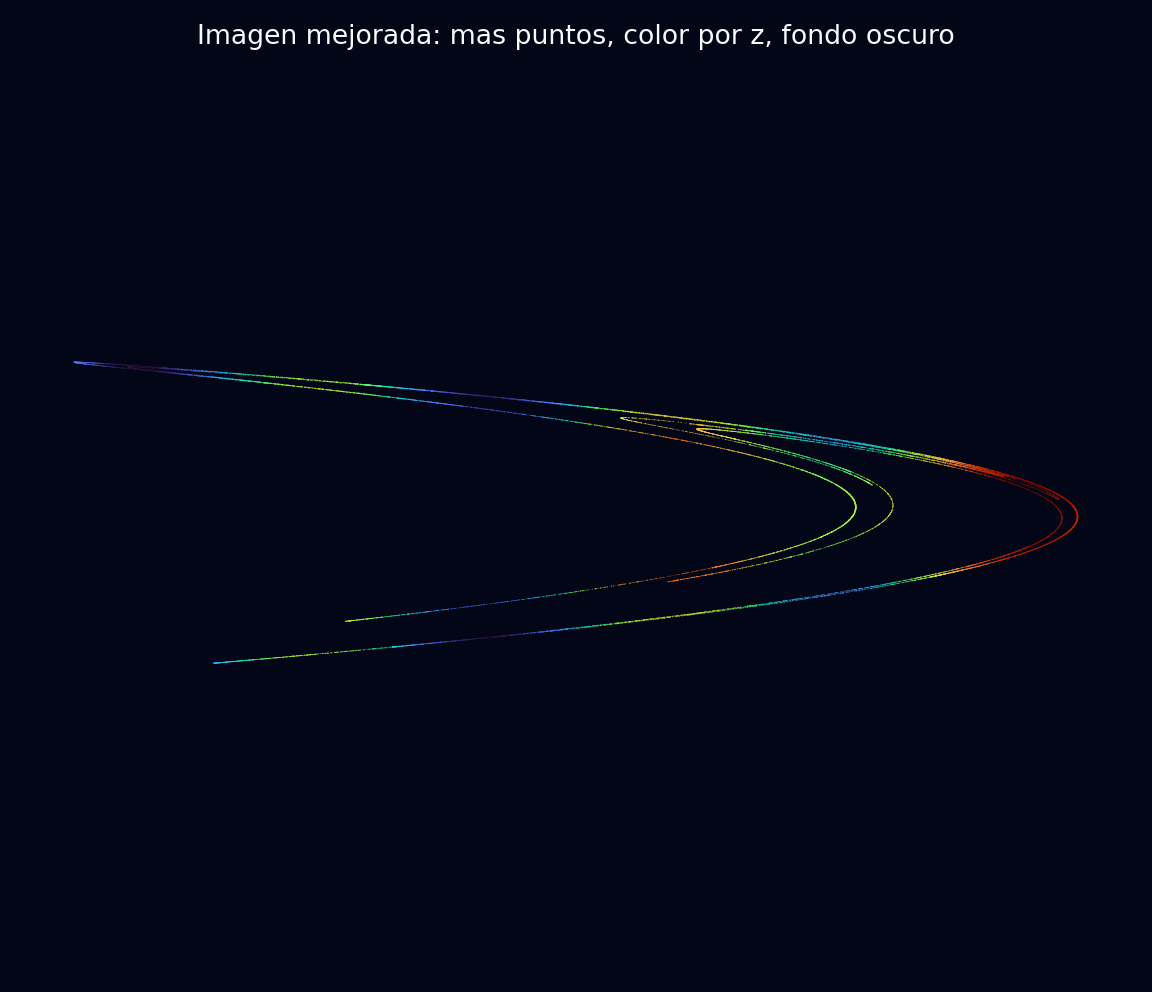
\includegraphics[width=0.48\linewidth]{images/generated/improved_dense_color_z.png}
\caption{Ejemplos generados por Chaos Toolbox: color por variable oculta y
mejora visual usando mas puntos, alpha bajo y fondo oscuro.}
\end{figure}

\begin{figure}[htbp]
\centering
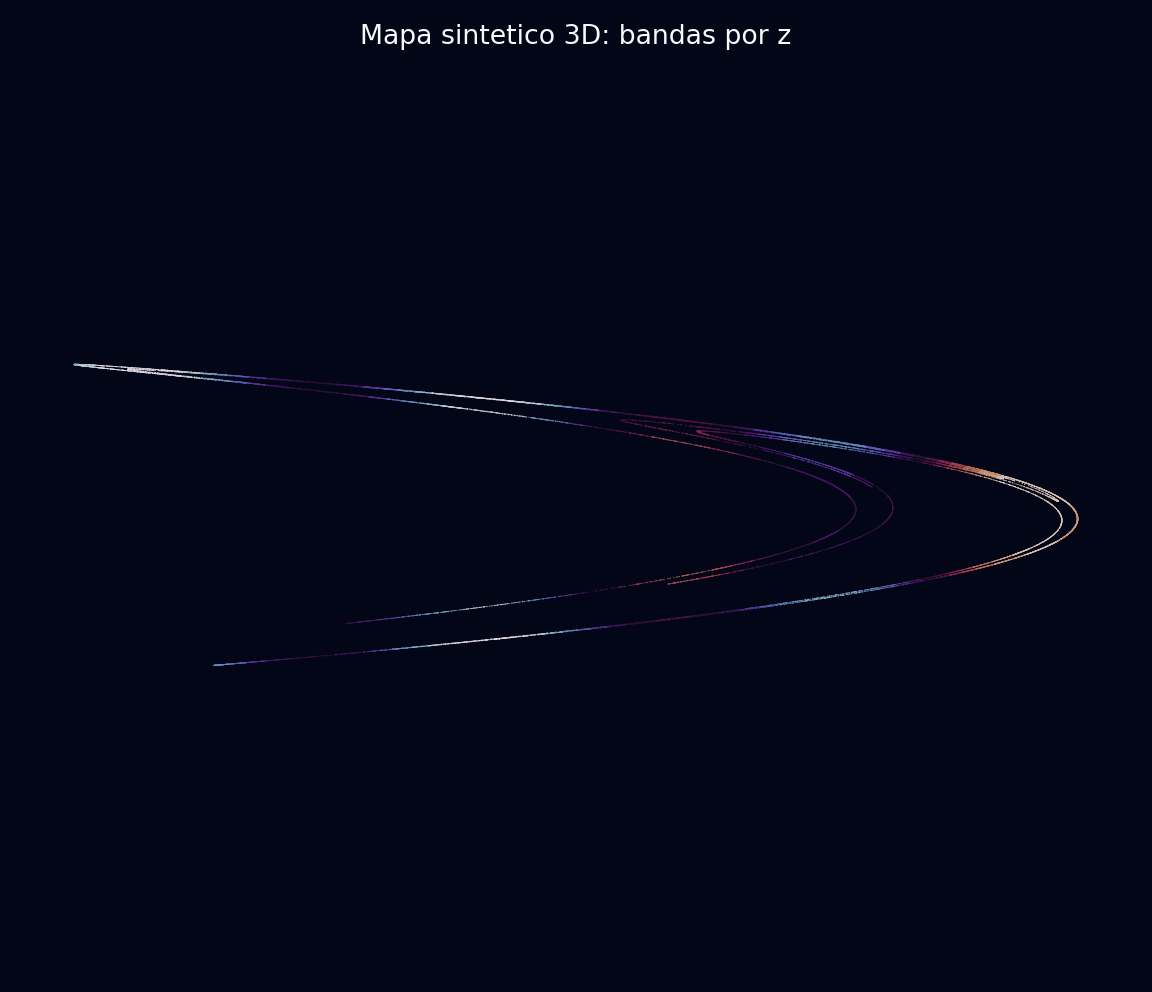
\includegraphics[width=0.48\linewidth]{images/generated/map3d_bands_z.png}
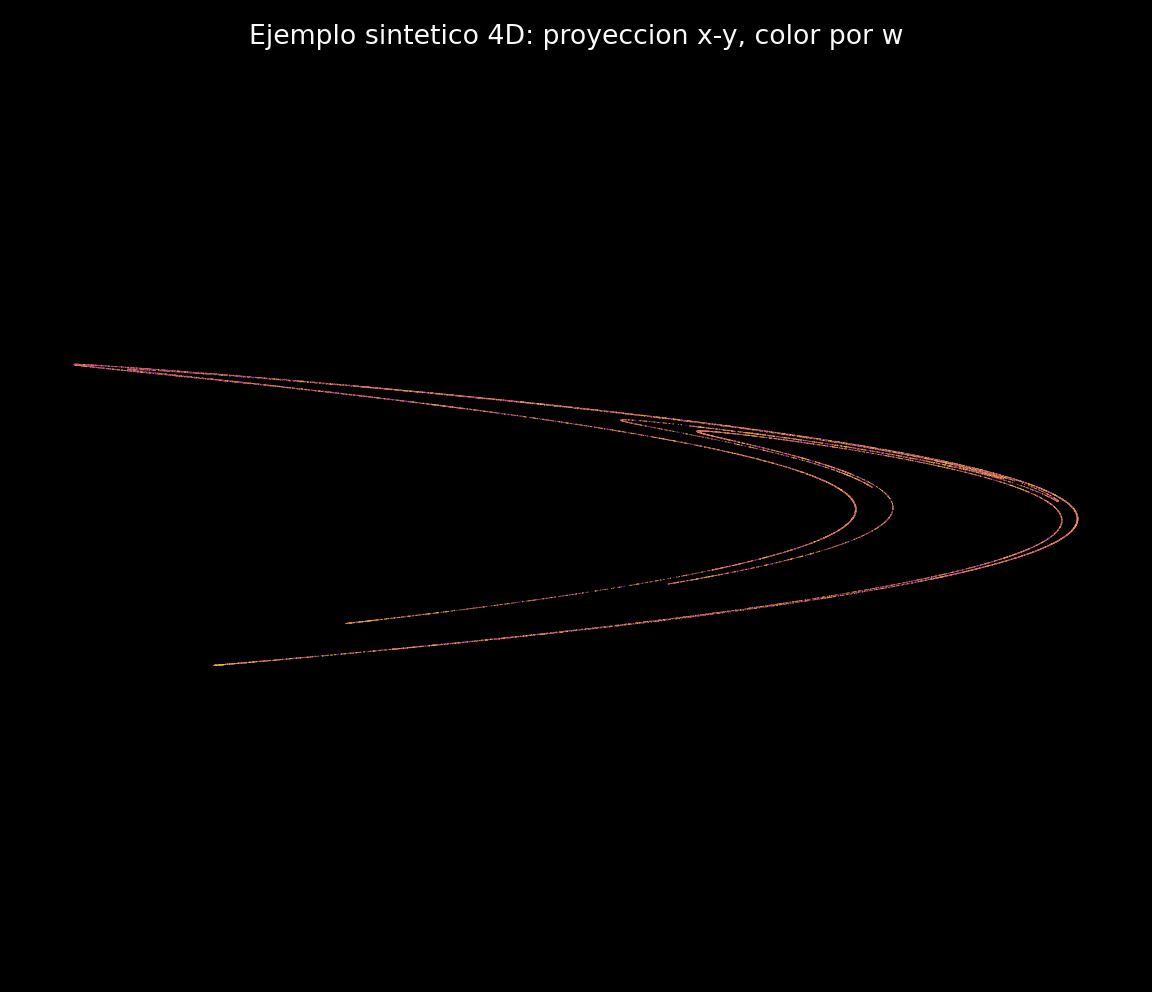
\includegraphics[width=0.48\linewidth]{images/generated/map4d_projection_w.png}
\caption{Bandas por coordenada sintetica y ejemplo 4D como proyeccion \(x-y\)
con color por \(w\).}
\end{figure}

\section{Codigos compactos}

El programa historico de Sprott codificaba familias de ecuaciones y coeficientes
en cadenas compactas. La reimplementacion educativa conserva esa idea: la
primera letra selecciona familia, dimension, tipo y orden; las letras
siguientes se leen como coeficientes.
\[
c=\frac{\operatorname{ord}(\chi)-77}{10}.
\]
Asi, \(\chi=M\) produce \(c=0\); letras antes de \(M\) producen coeficientes
negativos; letras despues de \(M\) producen coeficientes positivos.

\subsection{Family letters}

\begin{center}
\begin{tabular}{llll}
\toprule
Letras & Tipo & Dimension & Ordenes \\
\midrule
A--D & mapa polinomial & 1 & 2, 3, 4, 5 \\
E--H & mapa polinomial & 2 & 2, 3, 4, 5 \\
I--L & mapa polinomial & 3 & 2, 3, 4, 5 \\
M--P & mapa polinomial & 4 & 2, 3, 4, 5 \\
Q--T & flujo polinomial & 3 & 2, 3, 4, 5 \\
U--X & flujo polinomial & 4 & 2, 3, 4, 5 \\
Y--Z & funciones especiales & pendiente & pendiente \\
\bottomrule
\end{tabular}
\end{center}

Dentro de cada grupo de cuatro letras, la primera letra significa orden 2, la
segunda orden 3, la tercera orden 4 y la cuarta orden 5.

\section{Busqueda automatica}

El patron de busqueda de Sprott es experimental: generar muchas reglas simples,
simularlas, descartar las triviales y estudiar las candidatas. En esta app el
boton \emph{Buscar candidato} aplica filtros rapidos:
\begin{itemize}
  \item rechaza trayectorias divergentes o con valores no finitos;
  \item rechaza colapso a punto fijo;
  \item marca como baja complejidad las colas con poca dispersion o muchos
        estados repetidos;
  \item etiqueta como \code{candidate\_chaotic} solo a una trayectoria acotada y
        no colapsada.
\end{itemize}

Esa etiqueta no es una demostracion de caos. Para afirmar caos hacen falta
diagnosticos mas fuertes, por ejemplo exponentes de Lyapunov, espectro,
secciones, dimension y pruebas de sensibilidad con integracion mas larga.

\section{Reproduccion de figuras}

Desde la raiz del repositorio:
\[
\code{python assets/sprott/generate\_theory\_figures.py}
\]
El script escribe las imagenes en \code{assets/sprott/images/} y usa parametros
fijos para que este PDF sea reproducible.

\begin{thebibliography}{9}
\bibitem{sprott1993book}
J. C. Sprott, \emph{Strange Attractors: Creating Patterns in Chaos}, M\&T
Books, 1993.

\bibitem{sprott1993online}
J. C. Sprott, \emph{Strange Attractors: Creating Patterns in Chaos}, manuscrito
oficial en linea, University of Wisconsin,
\url{https://sprott.physics.wisc.edu/fractals/booktext/SABOOK.HTM}.

\bibitem{sprottgallery}
J. C. Sprott, \emph{Sprott's Fractal Gallery}, University of Wisconsin,
\url{https://sprott.physics.wisc.edu/FRACTALS.HTM}.

\bibitem{sprott1994flows}
J. C. Sprott, ``Some simple chaotic flows,'' \emph{Physical Review E}, vol. 50,
pp. R647--R650, 1994. DOI: \url{https://doi.org/10.1103/PhysRevE.50.R647}.
\end{thebibliography}

\end{document}
